\documentclass[12pt,a4paper]{article}
\usepackage[margin=2.35cm]{geometry}
\usepackage{fontspec}
\setmainfont{Times New Roman}
\usepackage{polyglossia}
\setdefaultlanguage{vietnamese}
\usepackage{graphicx}
\usepackage{booktabs}
\usepackage{array}
\usepackage{longtable}
\usepackage{enumitem}
\usepackage{tabularx}
\usepackage{titlesec}
\usepackage{hyperref}
\hypersetup{colorlinks=true,linkcolor=black,urlcolor=blue}
\setlength{\parindent}{0pt}
\setlength{\parskip}{5pt}
\setlength{\emergencystretch}{2em}
\raggedbottom
\newcolumntype{Y}{>{\raggedright\arraybackslash}X}
\setlist{leftmargin=1.5em,itemsep=3pt,topsep=4pt}
\titleformat{\section}{\large\bfseries}{\thesection.}{0.6em}{}
\titleformat{\subsection}{\normalsize\bfseries}{\thesubsection.}{0.6em}{}
\renewcommand{\contentsname}{Mục lục}
\graphicspath{{../figures/}}

\begin{document}
\begin{titlepage}
\begin{center}
{\large \textbf{ĐẠI HỌC QUỐC GIA THÀNH PHỐ HỒ CHÍ MINH}}\\
{\large \textbf{TRƯỜNG ĐẠI HỌC CÔNG NGHỆ THÔNG TIN}}\\[3.5cm]
{\Large \textbf{ĐỀ XUẤT Ý TƯỞNG ĐỒ ÁN MÔN HỌC CS114}}\\[0.5cm]
{\Large \textbf{ĐỀ TÀI:}}\\[0.5cm]
{\Large \textbf{ỨNG DỤNG HỌC MÁY DỰ ĐOÁN XU HƯỚNG VÀ GIÁ ĐÓNG CỬA CỔ PHIẾU FPT Ở PHIÊN KẾ TIẾP}}\\[1.4cm]
\end{center}

\begin{center}
\renewcommand{\arraystretch}{1.25}
\begin{tabular}{cll}
\toprule
\textbf{STT} & \textbf{Họ và tên} & \textbf{MSSV}\\
\midrule
1 & Lê Vũ Thiêm Hoàng & 25520584\\
2 & Nguyễn Tấn Dũng & 25520367\\
3 & Lưu Hoàng Minh Duy & 25520424\\
\bottomrule
\end{tabular}
\par\vspace{0.7cm}
\end{center}

\vfill
\begin{center}\textbf{THÀNH PHỐ HỒ CHÍ MINH, NĂM 2026}\end{center}
\end{titlepage}

\tableofcontents
\newpage

\section{Đặt vấn đề}
Giá cổ phiếu thay đổi theo thông tin doanh nghiệp, cung cầu và điều kiện kinh tế. Với dữ liệu đến hết một phiên giao dịch, nhóm đặt câu hỏi liệu các mô hình học máy có thể dự đoán hướng tăng/giảm và giá đóng cửa của phiên FPT kế tiếp hay không. Bài toán có đầu vào, nhãn và quy trình đánh giá cụ thể, phù hợp để thực hành tiền xử lý chuỗi thời gian, học có giám sát và đánh giá mô hình trong học phần CS114.

Đề tài so sánh hai cách tạo đầu vào. Nhánh 1 dùng giá và khối lượng giao dịch FPT cùng các chỉ báo kỹ thuật. Nhánh 2 bổ sung tỷ giá USD/VND, giá vàng quy đổi, CPI, GDP, chỉ số ngành ICT và các chỉ tiêu báo cáo tài chính FPT. Dữ liệu có tần suất tháng, quý hoặc năm chỉ được dùng sau ngày có thể biết để tránh đưa thông tin tương lai vào mô hình. Hệ thống là thử nghiệm học thuật hỗ trợ phân tích định lượng, không thay thế quyết định đầu tư.

\section{Mục tiêu của đề tài}
Mục tiêu chung là xây dựng pipeline tái lập được để dự báo một phiên giao dịch kế tiếp của FPT và đo tác động của các nhóm dữ liệu đầu vào.
\begin{enumerate}[label=\arabic*.]
\item Khảo sát OHLCV (Open, High, Low, Close, Volume) của cổ phiếu FPT và dữ liệu bổ trợ trong giai đoạn 2007--30/09/2025.
\item Chuẩn hóa dữ liệu, tạo đặc trưng chỉ từ thông tin đã có tại cuối phiên và căn dữ liệu tần suất thấp theo ngày có hiệu lực.
\item Huấn luyện, đánh giá các mô hình phân loại hướng và hồi quy giá bằng chia tập thời gian Train 85\% và Test 15\%.
\item So sánh hai nhánh đầu vào, phân tích sai số, giới hạn và các trường hợp dự báo sai.
\end{enumerate}

\section{Phạm vi và đối tượng nghiên cứu}
Đối tượng là mã FPT trên sàn chứng khoán HOSE. Dữ liệu OHLCV dừng tại 30/09/2025 để giữ mốc dữ liệu đồng bộ với các nguồn vĩ mô và báo cáo tài chính đã kiểm tra được. Mỗi hàng ở cuối phiên $t$ dự báo phiên giao dịch quan sát được kế tiếp $t+1$. Bài toán phân loại có nhãn Tăng hoặc Giảm theo giá đóng cửa; phiên không đổi bị loại khỏi chấm điểm phân loại. Bài toán hồi quy giữ cả phiên không đổi và dự báo giá đóng cửa ở $t+1$.

\newpage
\section{Đầu vào và đầu ra dự kiến}
\subsection{Đầu vào}
{\small\renewcommand{\arraystretch}{1.12}
\begin{tabularx}{\textwidth}{@{}>{\raggedright\arraybackslash}p{2.6cm}>{\raggedright\arraybackslash}p{5.0cm}Y@{}}
\toprule
\textbf{Nhóm} & \textbf{Biến} & \textbf{Cách dùng}\\\midrule
Giao dịch FPT & open, high, low, close, volume & Tạo lợi nhuận trễ, SMA/EMA, RSI, MACD, Bollinger, biến động và đặc trưng nến.\\
Vĩ mô & USD/VND, CPI, GDP, vàng quy đổi VND & Ghép lùi từ ngày dữ liệu được công bố hoặc có hiệu lực.\\
Ngành ICT & Vốn hóa, P/E, Absolute P/E & Snapshot theo ngày quan sát, chỉ dùng từ phiên sau.\\
Tài chính FPT & Doanh thu thuần, lợi nhuận gộp, EBIT, lợi nhuận sau thuế cổ đông công ty mẹ, số cổ phiếu lưu hành & EBIT bằng lợi nhuận trước thuế cộng chi phí lãi vay. Số cổ phiếu dùng từ ngày hiệu lực đã xác minh.\\
\bottomrule
\end{tabularx}}

Các nguồn dự kiến gồm VCI/Vietcap qua vnstock cho giá cổ phiếu FPT; Investing.com cho tỷ giá, vàng và CPI; World Bank cho GDP năm; Simply Wall St cho các snapshot ngành công nghệ Việt Nam. Nhóm sẽ lưu nguồn, đơn vị, khoảng thời gian và ngày có hiệu lực của từng chuỗi. Giá vàng quy đổi bằng giá XAU/USD nhân USD/VND, có đơn vị VND trên một ounce vàng; đây không phải giá vàng miếng trong nước. GDP dùng số liệu thực tế đã công bố, không trộn với dự báo. Chỉ tiêu chưa đủ độ phủ hoặc chưa xác minh được ngày công bố sẽ được ghi rõ trong báo cáo thực nghiệm.

\subsection{Đầu ra}
{\small\renewcommand{\arraystretch}{1.12}
\begin{tabularx}{\textwidth}{@{}>{\raggedright\arraybackslash}p{4cm}Y@{}}
\toprule
Target session & Phiên giao dịch FPT kế tiếp.\\
Predicted direction & Tăng hoặc Giảm.\\
Confidence score & Xác suất dự đoán lớp Tăng trong hai lớp Tăng/Giảm.\\
Predicted close price & Giá đóng cửa ước tính, đơn vị nghìn VND/cổ phiếu.\\
Key signals & Nhánh đặc trưng và mô hình tạo dự báo.\\
\bottomrule
\end{tabularx}}

\begin{center}
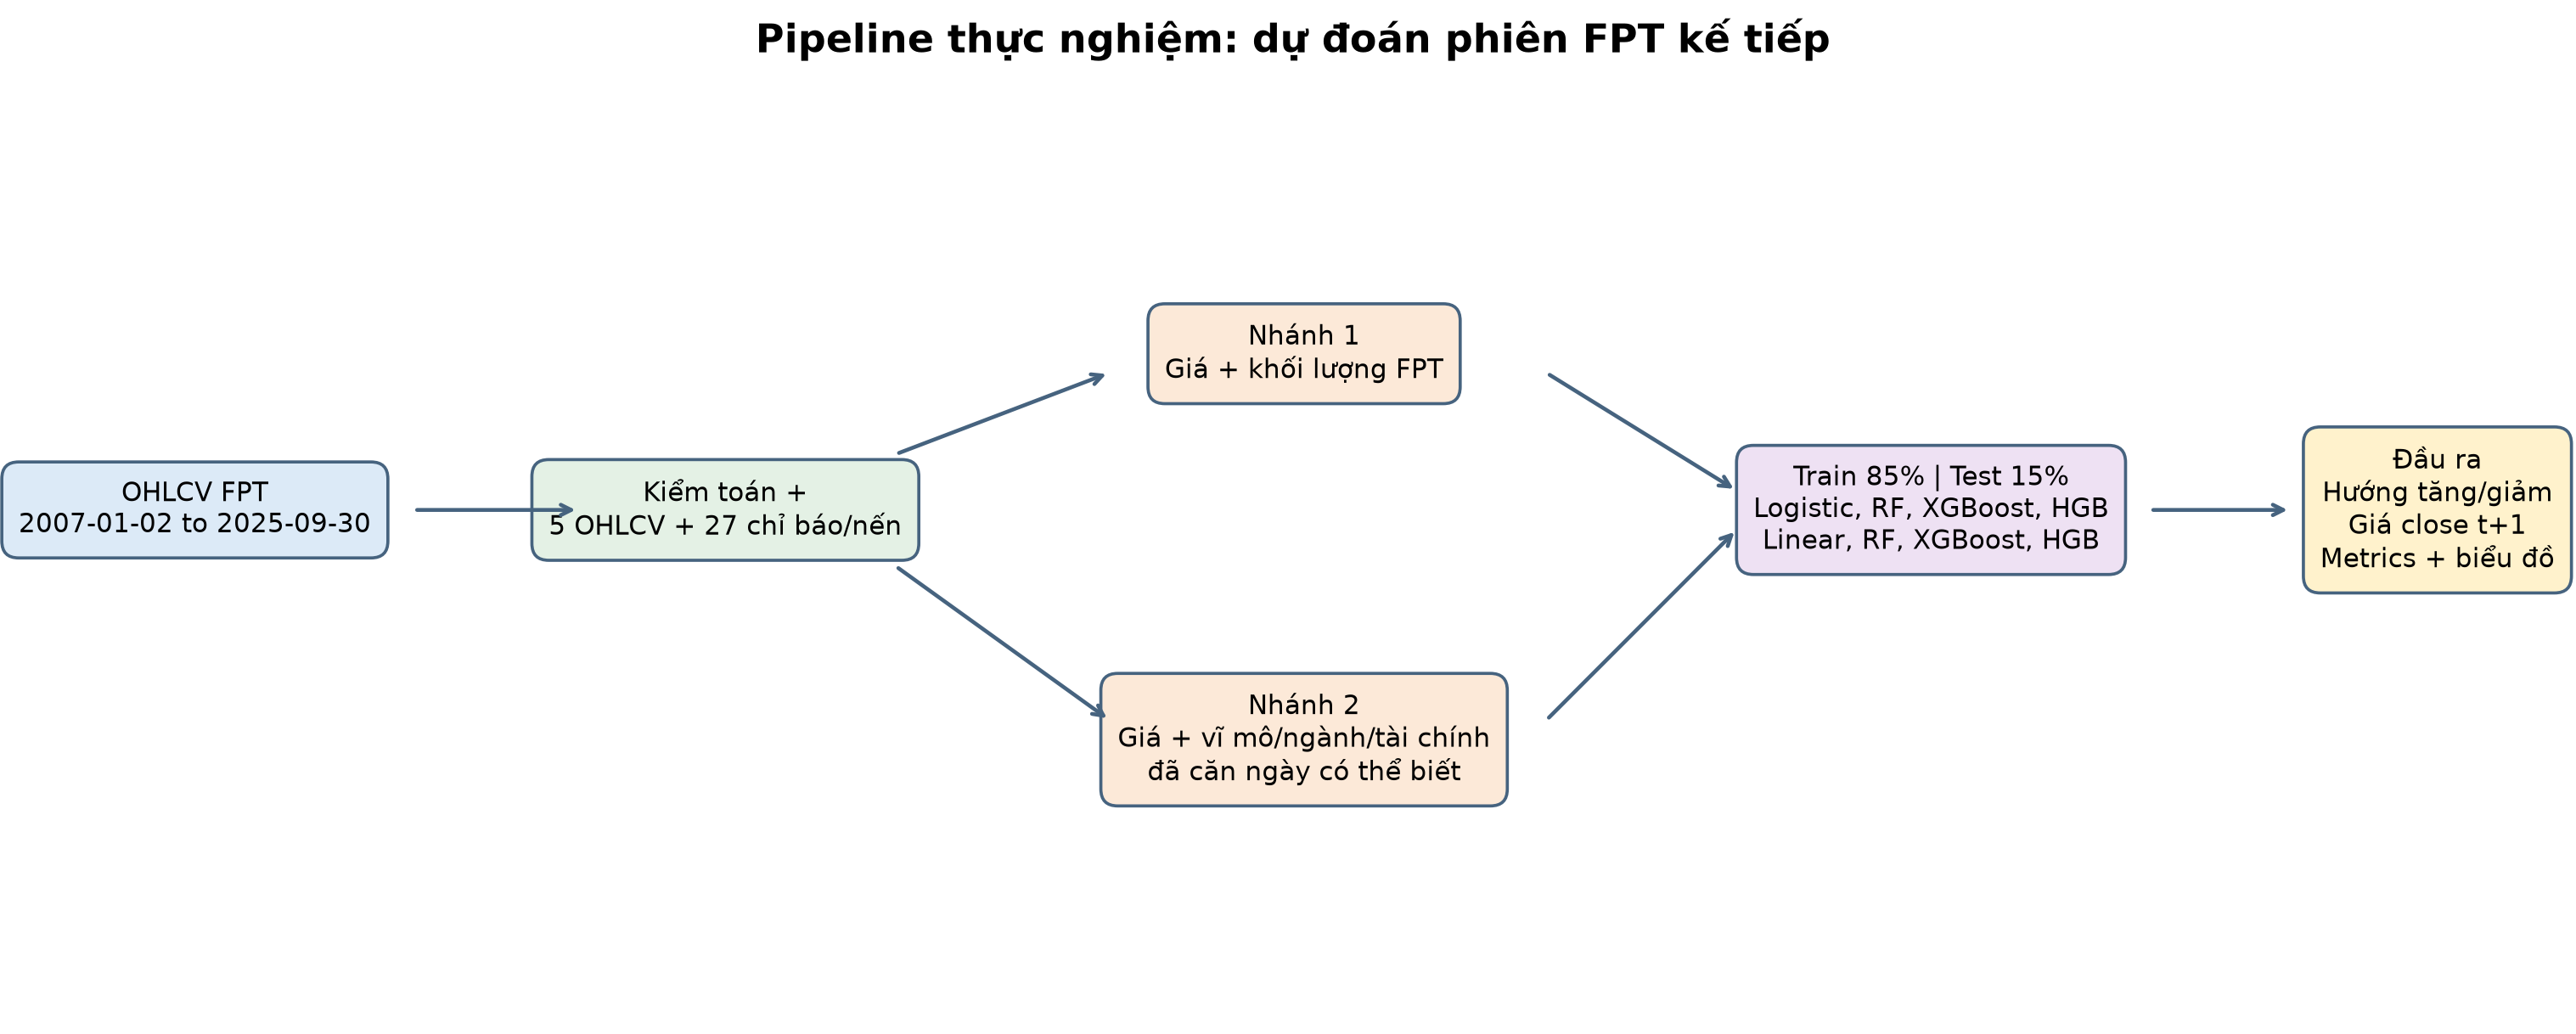
\includegraphics[width=\textwidth]{00_pipeline_overview.png}
\end{center}

\newpage
\section{Hướng tiếp cận và công nghệ dự kiến}
Nhóm dùng Python, pandas, NumPy, scikit-learn, XGBoost, matplotlib, joblib và vnstock. Đặc trưng giá chỉ dùng hiện tại và quá khứ. Dữ liệu bổ trợ được ghép từ ngày công bố hoặc ngày có hiệu lực mô phỏng, không điền ngược. Khi thiếu lịch công bố, nhóm giả định trễ 45 ngày sau cuối quý cho báo cáo tài chính và 180 ngày sau cuối năm cho GDP. Đây là giả định thực nghiệm, chưa đảm bảo khôi phục đầy đủ phiên bản dữ liệu từng biết trong quá khứ. StandardScaler nằm trong Pipeline của mô hình tuyến tính nên chỉ học tham số chuẩn hóa từ Train.

Nhánh 1 dùng 5 trường OHLCV gốc và 27 đặc trưng kỹ thuật/nến, tổng cộng 32 biến. Nhánh 2 bổ sung 12 biến vĩ mô, ngành và tài chính, gồm lịch sử số cổ phiếu lưu hành, thành 44 biến. Hai nhánh dùng cùng các ngày hợp lệ, cùng nhãn và cùng ranh giới Train/Test. Nhóm kiểm tra độ phủ từng chuỗi trước khi xác định cửa sổ chung.

Các mô hình phân loại gồm Majority Baseline, Logistic Regression, Random Forest, XGBoost Classifier và HistGradientBoosting. Các mô hình hồi quy gồm Last-Close Baseline, Linear Regression, Random Forest Regressor, XGBoost Regressor và HistGradientBoosting Regressor. Baseline đơn giản được giữ để biết mô hình phức tạp có thực sự cải thiện hay không.

\section{Cách đánh giá dự kiến}
Tập dữ liệu được sắp theo ngày mục tiêu. 85\% hàng đầu là Train, 15\% cuối là Test, không xáo trộn. Test kết thúc tại phiên 30/09/2025. Ngày bắt đầu và số mẫu thực tế của cửa sổ so sánh chung được ghi trong báo cáo sau khi kiểm tra độ phủ dữ liệu. Mọi mô hình được huấn luyện trên Train trước khi dự báo Test.

{\small\renewcommand{\arraystretch}{1.12}
\begin{tabularx}{\textwidth}{@{}>{\raggedright\arraybackslash}p{4cm}Y@{}}
\toprule
\textbf{Thuật ngữ} & \textbf{Ý nghĩa}\\\midrule
Giá đóng cửa (close) & Giá giao dịch cuối cùng của một phiên, đơn vị nghìn VND/cổ phiếu trong snapshot.\\
Accuracy & Tỷ lệ dự đoán đúng hướng trên tổng số phiên.\\
Balanced Accuracy & Trung bình tỷ lệ đoán đúng hai lớp Tăng và Giảm.\\
Precision, Recall & Tỷ lệ phiên thật sự Tăng trong số phiên dự báo Tăng và tỷ lệ nhận đúng trong số phiên thật sự Tăng.\\
F1-score & Trung bình điều hòa giữa Precision và Recall của lớp Tăng.\\
ROC-AUC & Khả năng xếp hạng phiên Tăng cao hơn phiên Giảm theo xác suất.\\
MAE, RMSE, MAPE & MAE và RMSE đo sai số theo đơn vị giá; MAPE đo sai số tương đối theo phần trăm.\\
Tolerance Accuracy & Tỷ lệ dự báo giá nằm trong ngưỡng $\pm0.5\%$, $\pm1.0\%$, $\pm2.0\%$ so với giá thực tế.\\
Directional Accuracy & Tỷ lệ dự đoán đúng chiều thay đổi suy ra từ giá dự báo.\\
\bottomrule
\end{tabularx}}

Nhóm xuất bảng metric, confusion matrix, biểu đồ Actual Close so với Predicted Close của từng mô hình, biểu đồ so sánh XGBoost hai nhánh có cửa sổ phóng to 80 phiên và biểu đồ cột các metric giữa hai nhánh.

Phân loại hướng và hồi quy giá được chấm riêng. Nếu dùng kết quả Test để đánh dấu mô hình tốt nhất, nhóm sẽ trình bày đây là lựa chọn phục vụ minh họa sau thực nghiệm; điểm của mô hình được chọn không còn là đánh giá độc lập hoàn toàn. Sau khi ghi kết quả, mô hình minh họa có thể học lại trên toàn bộ nhãn đã có để tạo dự báo mới nhất.

\newpage
\section{Kết quả dự kiến}
Sản phẩm dự kiến gồm pipeline dữ liệu tái lập được, bảng đặc trưng và kiểm toán dữ liệu, mô hình đã huấn luyện kèm lệnh dự báo phiên kế tiếp, cùng báo cáo thực nghiệm hai nhánh. Các kết quả hiện có sẽ được dùng để phân tích trường hợp thêm dữ liệu bổ trợ có cải thiện hay làm giảm hiệu quả dự báo. Nhóm sẽ báo cáo cả kết quả không cải thiện thay vì chỉ chọn mô hình có chỉ số cao.

\end{document}
